\setcounter{chapter}{1}
\setcounter{section}{1}
\chapter{\tenchuongii}
%===================================================================
Từ mạng CNN cơ bản người ta có thể tạo ra rất nhiều mô hình khác nhau, từ những mạng neural cơ bản 1 đến 2 layer đến 100 layer. Khi thêm nhiều layer hơn thì theo lý thuyết độ chính xác phải cao hơn, nhưng thực tế lại không phải độ chính xác không tăng thậm chí là có lúc lại giảm. Về kernel ta có 3x3, 5x5 hay thậm chí 7x7, vậy thì dùng kernel nào tốt, càng nhỏ liệu có càng chính xác? Vì vậy, chương này ta sẽ tìm hiểu một số mô hình nổi tiếng của CNN, các cài đặt, cấu hình của chúng và hướng áp dụng vào bài toán chuẩn đoán bệnh lao của luận văn.

\section{Mô hình VGG-16}
\subsection{Mô hình VGG16 là gì}
VGG là viết tắt của Visual Geometry Group; nó là một kiến trúc CNN sâu tiêu chuẩn với nhiều lớp. Karen Simonyan và Andrew Zisserman \cite{vgg16} đã đề xuất ý tưởng về mạng VGG vào năm 2013 và gửi mô hình thực tế dựa trên ý tưởng này trong ImageNet Challenge 2014. Họ gọi nó là VGG theo tên bộ phận của Visual Geometry Group tại Đại học Oxford nơi họ làm việc.

\subsection{Cấu hình mô hình VGG16}
Trong tất cả các cấu hình, VGG16 được xác định là mô hình hoạt động tốt nhất trên tập dữ liệu ImageNet. Hãy xem lại kiến trúc thực tế của cấu hình này (Hình \ref{fig:vgg16_imagenet}).
Đầu vào cho bất kỳ cấu hình mạng nào được coi là hình ảnh có kích thước cố định 224 x 224 với ba kênh R, G và B. Quá trình xử lý trước duy nhất được thực hiện là chuẩn hóa các giá trị RGB cho mỗi pixel. Điều này đạt được bằng cách trừ đi giá trị trung bình cho mỗi pixel.

Hình ảnh được chuyển qua ngăn xếp đầu tiên gồm 2 lớp tích chập có kích thước tiếp nhận rất nhỏ là 3 x 3, tiếp theo là kích hoạt ReLU. Mỗi lớp trong số hai lớp này chứa 64 bộ lọc. Stride được cố định ở 1 pixel và padding là 1 pixel. Cấu hình này bảo toàn độ phân giải không gian và kích thước của bản đồ kích hoạt đầu ra giống với kích thước hình ảnh đầu vào. Các bản đồ kích hoạt sau đó được chuyển qua tổng hợp tối đa không gian trên cửa sổ 2 x 2 pixel, với stride là 2 pixel. Điều này làm giảm một nửa kích thước của các lần kích hoạt. Do đó, kích thước của các kích hoạt ở cuối ngăn xếp đầu tiên là 112 x 112 x 64.

Các kích hoạt sau đó chảy qua ngăn xếp thứ hai tương tự, nhưng với 128 bộ lọc so với 64 bộ lọc trong ngăn xếp thứ nhất. Do đó, kích thước sau ngăn xếp thứ hai trở thành 56 x 56 x 128. Tiếp theo là ngăn xếp thứ ba với ba lớp chập và một lớp tổng hợp tối đa. Số lượng bộ lọc được áp dụng ở đây là 256, làm cho kích thước đầu ra của ngăn xếp là 28 x 28 x 256. Tiếp theo là hai ngăn xếp gồm ba lớp chập, với mỗi ngăn chứa 512 bộ lọc. Đầu ra ở cuối cả hai ngăn xếp này sẽ là 7 x 7 x 512.

Các chồng lớp chập trùng được theo sau bởi ba lớp được kết nối hoàn chỉnh với một lớp làm phẳng ở giữa. Hai lớp đầu tiên có 4.096 tế bào thần kinh mỗi lớp và lớp được kết nối đầy đủ cuối cùng đóng vai trò là lớp đầu ra và có 1.000 tế bào thần kinh tương ứng với 1.000 lớp có thể có cho tập dữ liệu ImageNet. Tiếp theo là lớp đầu ra là lớp kích hoạt Softmax được sử dụng để phân loại (Hình \ref{fig:vgg16_imagenet_detail}).

\begin{figure}[H]
	\centering
	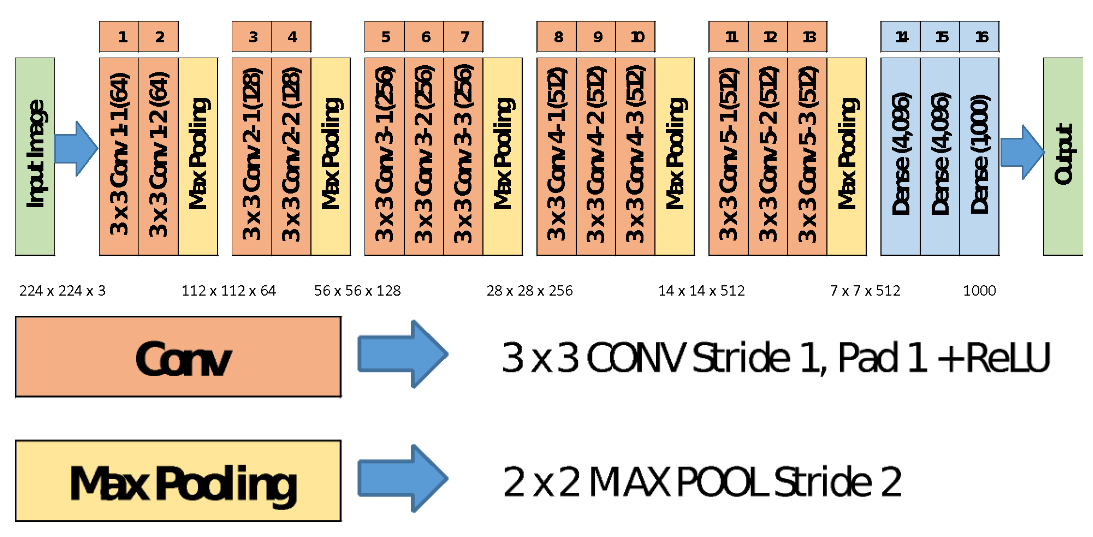
\includegraphics[width=1\linewidth]{images/vgg16_imagenet_detail}
	\caption{Chi tiết kiến trúc VGG16.}
	\label{fig:vgg16_imagenet_detail}
\end{figure}

\subsection{Ưu nhược điểm của mô hình VGG16}
\textbf{Ưu điểm:}
\begin{itemize}
	\item VGG đã mang đến một sự cải tiến lớn về độ chính xác và cải thiện cả về tốc độ. Điều này chủ yếu là do cải thiện độ sâu của mô hình.
	\item Sự gia tăng số lượng các lớp với các hạt nhân nhỏ hơn làm tăng tính phi tuyến tính, điều này luôn luôn là một điều tích cực trong học sâu.
	\item VGG mang theo nhiều kiến trúc khác nhau được xây dựng dựa trên khái niệm tương tự. Điều này cung cấp cho chúng ta nhiều lựa chọn hơn về kiến trúc nào có thể phù hợp nhất với ứng dụng của chúng ta.
\end{itemize}
\textbf{Nhược điểm:}
\begin{itemize}
	\item Một vấn đề của VGG liên quan đến giới hạn tính toán của máy tính cũng khiến cho việc huấn luyện không hiệu quả khi số lượng hidden layers lớn lên. Vấn đề này có tên là vanishing gradient.
	\item Số lượng bộ lọc mà chúng ta có thể sử dụng tăng gấp đôi trên mỗi bước hoặc qua mỗi ngăn xếp của lớp tích chập. Đây là một nguyên tắc chính được sử dụng để thiết kế kiến trúc của mạng VGG16. Một trong những nhược điểm quan trọng của mạng VGG16 là nó là một mạng khổng lồ, có nghĩa là cần nhiều thời gian hơn để đào tạo các tham số của nó.
\end{itemize}


\section{Mô hình ResNet}
\subsection{Mô hình Resnet là gì}
ResNet (Residual Network) được Kaiming He\cite{resnet} giới thiệu đến công chúng vào năm 2015, hiện tại thì có rất nhiều biến thể của kiến trúc ResNet với số lớp khác nhau như ResNet-18, ResNet-34, ResNet-50, ResNet-101, ResNet-152,... với tên là ResNet theo sau là một số chỉ kiến trúc ResNet với số lớp nhất định.

Các kiến trúc mạng trước khi Resnet ra đời như Alexnet, VGG được coi là các mạng nơ ron thuần (plain network). Đối với các mạng nơ ron thuần, Kaiming He\cite{resnet} đã thí nghiệm và đưa ra kết luận khi tăng số lượng layer của mạng từ 20 lên 56 thì lỗi trên tập huấn luyện và trên tập kiểm tra của mạng 56 layer đều cao hơn so với mạng 20 layer(hình \ref{fig:resnet_vanishing_gradient}). 
\begin{figure}[H]
	\centering
	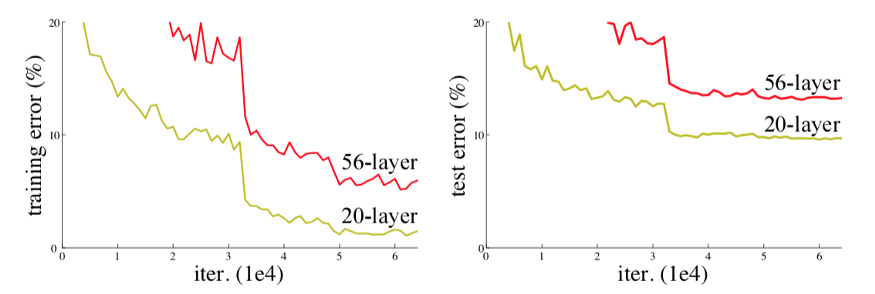
\includegraphics[width=1\linewidth]{images/resnet_vanishing_gradient}
	\caption{Lỗi huấn luyện và lỗi kiểm tra với mạng 20 layer và 56 layer.}
	\label{fig:resnet_vanishing_gradient}
\end{figure} 
ResNet đưa ra phương phán cho vấn đề trên là sử dụng kết nối "tắt" đồng nhất để xuyên qua một hay nhiều lớp. Một khối như vậy được gọi là một Residual Block(hình \ref{fig:resnet_residual_block}). Ý tưởng chính của phương pháp này thực ra rất đơn giản, Resnet thực hiện residual mapping để copy thông tin từ các layer nông shallow layer trước đó đến các layer sâu hơn. Chúng ta giả sử output của shallow layer là $x$. Trong quá trình forward của mạng nó được đưa qua một phép biến đổi tuyến tính $F(x)$. Chúng ta giả sử output của phép biến đổi tuyền tính này là $H(x)$. Một residual (phần dư) giữa deep layer và shallow layer là
$$\mathcal{F}(\mathbf{x}; W_i) := \mathcal{H}(\mathbf{x}) - \mathbf{x}$$
Trong đó, $W_i$ là các tham số của mô hình CNN với phép biến đổi $F$ và nó được tối ưu trong quá trình huấn luyện.
\begin{figure}[H]
	\centering
	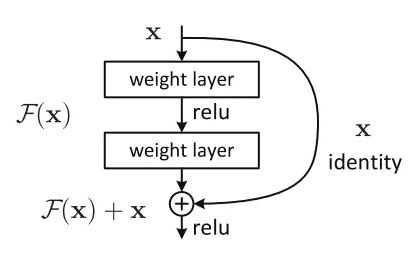
\includegraphics[width=0.5\linewidth]{images/resnet_residual_block}
	\caption{Residual block.}
	\label{fig:resnet_residual_block}
\end{figure}
Việc thêm vào các residual block vào trong kiến trúc mạng deep learning có hai cách tuỳ thuộc vào từng trường hợp cụ thể.
\begin{itemize}
	\item {\bf identity mapping} trong trường hợp này residual mapping đơn giản là việc cộng trực tiếp $x$ vào đầu ra của các stacked block $F(x)$. Đây là một cách sử dụng khá phổ biến trong thiết kế mạng ResNet nếu như input activation có cùng số chiều với output activation.
	\begin{figure}[H]
		\centering
		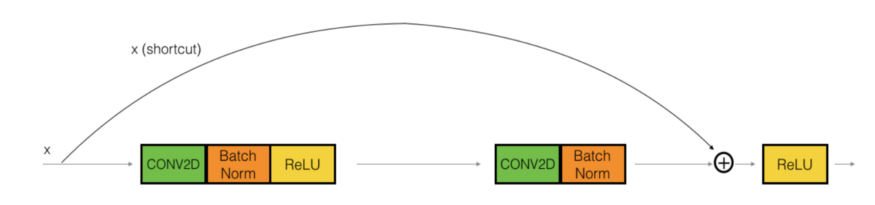
\includegraphics[width=1\linewidth]{images/resnet_identity_mapping}
		\caption{Identity mapping.}
		\label{fig:resnet_identity_mapping}
	\end{figure}
	\item {\bf Convolutional block} một trường hợp khác là thay vì cộng trực tiếp giá trị của input activation chúng ta sẽ đưa qua một convolution transformation. Trường hợp này có thể được thực hiện trong trường hợp input activation và output activation có số chiều khác nhau. Lúc này đầu ra được xác định như sau $y=F(x;Wi)+\text{Conv}(x)$.
	\begin{figure}[H]
		\centering
		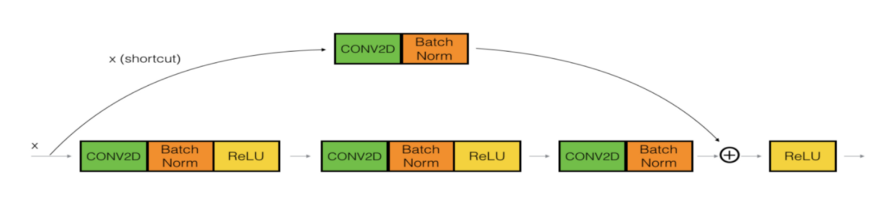
\includegraphics[width=1\linewidth]{images/resnet_conv_block}
		\caption{Convolutional block.}
		\label{fig:resnet_conv_block}
	\end{figure}
\end{itemize}
\subsection{Cấu hình của mô hình Resnet}
Hình \ref{fig:resnet_architecture} dưới đây mô tả chi tiết kiến trúc mạng nơ ron ResNet
\begin{figure}[H]
	\centering
	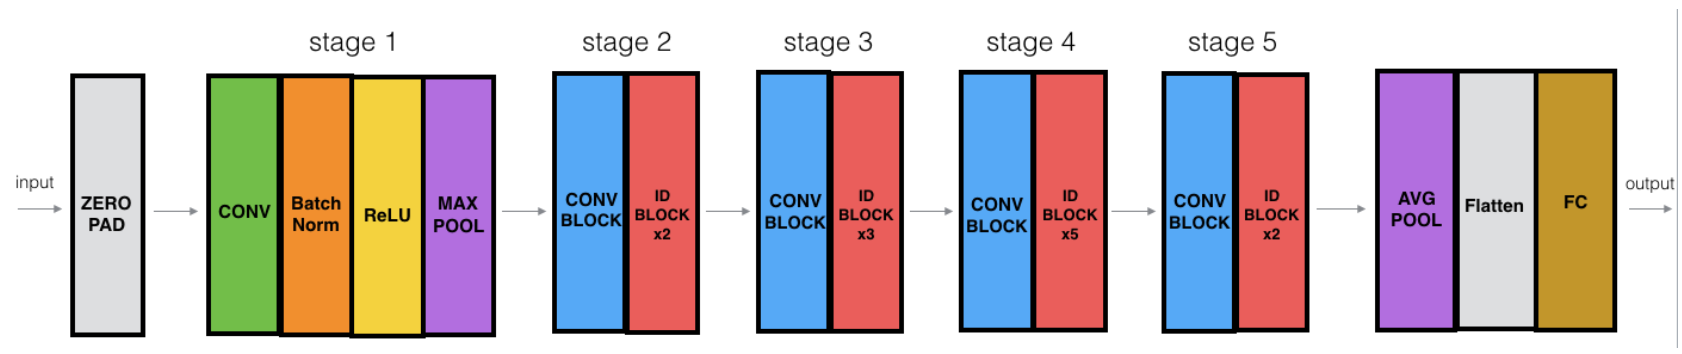
\includegraphics[width=1\linewidth]{images/resnet_architecture}
	\caption{Kiến trúc mạng ResNet.}
	\label{fig:resnet_architecture}
\end{figure}
"ID BLOCK" trong hình trên là viết tắt của từ Identity block và ID BLOCK x3 nghĩa là có 3 khối Identity block chồng lên nhau. Nội dung hình \ref{fig:resnet_architecture} như sau:
\begin{itemize}
	\item Zero-padding : Input với (3,3)
	\item Stage 1 : Tích chập (Conv1) với 64 filters với shape(7,7), sử dụng stride (2,2). BatchNorm, MaxPooling (3,3).
	\item Stage 2 : Convolutiontal block sử dụng 3 filter với size 64x64x256, f=3, s=1. Có 2 Identity blocks với filter size 64x64x256, f=3.
	\item Stage 3 : Convolutional sử dụng 3 filter size 128x128x512, f=3,s=2. Có 3 Identity blocks với filter size 128x128x512, f=3.
	\item Stage 4 : Convolutional sử dụng 3 filter size 256x256x1024, f=3,s=2. Có 5 Identity blocks với filter size 256x256x1024, f=3.
	\item Stage 5 :Convolutional sử dụng 3 filter size 512x512x2048, f=3,s=2. Có 2 Identity blocks với filter size 512x512x2048, f=3.
	\item The 2D Average Pooling : sử dụng với kích thước (2,2).
	\item The Flatten.
	\item Fully Connected (Dense) : sử dụng softmax activation.
\end{itemize}


\subsection{Ưu nhược điểm của mô hình ResNet}
\textbf{Ưu điểm:}
\begin{itemize}
	\item Kiến trúc ResNet không cần phải kích hoạt tất cả các nơ-ron trong mọi epoch (một epoch được tính là khi chúng ta đưa tất cả dữ liệu trong tập train vào mạng neural network 1 lần). Điều này làm giảm đáng kể thời gian đào tạo và cải thiện độ chính xác. Khi một đặc trưng đã được học, nó sẽ không cố gắng học lại mà tập trung vào việc học các đặc trưng mới hơn. Một cách tiếp cận rất thông minh đã cải thiện đáng kể hiệu suất đào tạo mô hình.
	\item ResNets giải quyết được khá tốt vấn đề Vanishing Gradient của các mạng CNN thuần.
	\item Có thể đào tạo dễ dàng các mạng với số lớp rất lớn mà không làm tăng tỷ lệ đào tạo lỗi.
\end{itemize}
\textbf{Nhược điểm: \cite{resnet_disadvantage}}
\begin{itemize}
	\item Đối với mạng sâu hơn, việc phát hiện lỗi trở nên khó khăn.
	\item Nếu mạng quá nông, việc đào tạo có thể rất kém hiệu quả.
\end{itemize}

\section{Mô hình DenseNet}
\subsection{Mô hình DenseNet là gì}
DenseNet - Dense Convolutional Network (Mạng Tích chập Kết nối Dày đặc) - là một trong những biến thể mở rộng của Resnet và là một kiến trúc mạng,trong đó mỗi lớp được kết nối trực tiếp với mỗi lớp khác nhau theo kiểu chuyển tiếp (trong mỗi khối dense block). Đối với mỗi lớp, các bản đồ đặc trưng (feature map) của tất cả các lớp ở phần trước được coi là các đầu vào riêng biệt và ở đó các bản đồ tính năng lại tiếp tục làm đầu vào cho tất cả các lớp tiếp theo. 

\begin{figure}[H]
	\centering
	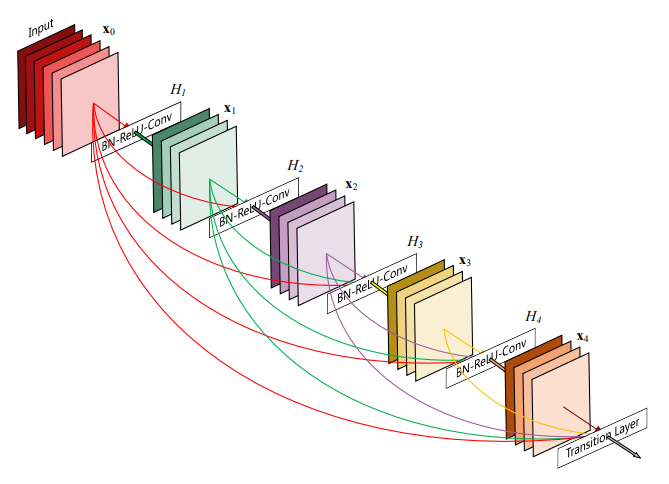
\includegraphics[width=0.8\linewidth]{images/densenet_hl}
	\caption{Kiến trúc DenseNet.}
	\label{fig:kien_truc_densenet}
\end{figure} 

Để cải thiện hơn nữa luồng thông tin giữa các lớp, DenseNet đề xuất một mô hình kết nối mà từ bất kỳ lớp nào cũng có thể kết nối đến tất cả các lớp tiếp theo. Hình \ref{fig:kien_truc_densenet} minh họa bố trí kiến trúc của DenseNet. Dễ dàng nhìn thấy, lớp thứ $l$ nhận được các bản đồ đặc trưng của tất cả các lớp trước đó, $x_0, x_1, x_2, . . . , x_{l-1}),$ làm đầu vào:
\begin{equation}\label{eq:denseconnectivity}
	x_l = H_l([x_0, x_1, . . . , x_{l-1}])
\end{equation}
với $[x_0, x_1, . . . , x{l-1}]$ đề cập đến việc nối các trích chọn đặc trưng được tạo thành trong các lớp $0, 1, ..., {l-1}$. Do khả năng kết nối dày đặc của nó, Gao Huang\cite{densenet} gọi kiến trúc mạng này là Mạng kết nối dày đặc (DenseNet). Để dễ thực hiện, DenseNet nối nhiều đầu vào của $H_l$(·) trong phương trình \ref{eq:denseconnectivity} thành một tensor duy nhất.\\
{\bf Hàm tổng hợp - Composite function}
Ta định nghĩa $H_l$(·) là một hàm tổng hợp của ba hoạt động liên tiếp: Batch Normalization (BN), tiếp theo là một hàm tinh chỉnh các đơn vị tuyến tính (ReLU) và một tích chập 3 × 3 (Conv).\\
{\bf Tầng hợp nhất - Pooling layers}
Thao tác nối được sử dụng trong Phương trình \ref{eq:denseconnectivity} không khả thi khi kích thước của bản đồ đối tượng thay đổi. Tuy nhiên, một phần thiết yếu của mạng tích chập là các lớp lấy mẫu xuống làm thay đổi kích thước của bản đồ đối tượng. Để tạo điều kiện thuận lợi cho việc giảm tần số lấy mẫu trong kiến trúc, DenseNet chia mạng thành nhiều khối dày đặc được kết nối với nhau(hình \ref{fig:densenet_3blk}). DensetNet đề cập đến các lớp giữa các khối là các lớp chuyển tiếp, các lớp này thực hiện tích chập và tổng hợp. Các lớp chuyển tiếp được sử dụng trong các cấu trúc DenseNet bao gồm lớp chuẩn hóa hàng loạt và lớp tích chập 1 × 1, tiếp theo là lớp gộp trung bình 2 × 2.
\begin{figure}[H]
	\centering
	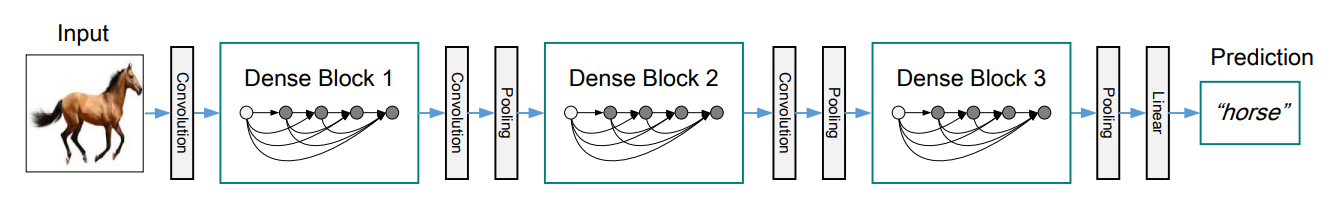
\includegraphics[width=1\linewidth]{images/densenet_3blk}
	\caption{Một DenseNet sâu với ba khối dày đặc.}
	\label{fig:densenet_3blk}
\end{figure}
{\bf Tỉ lệ phát triển - Growth rate}
Nếu mỗi hàm $H_l$ tạo ra $k$ bản đồ đặc trưng, thì lớp thứ $l$ có $k_0 + k{l-1}$ bản đồ đặc trưng đầu vào, trong đó $k_0$ là số kênh trong lớp đầu vào. Một điểm khác biệt quan trọng giữa DenseNet và các kiến trúc mạng trước đó là DenseNet có thể có các lớp rất hẹp, ví dụ: $k = 12$. Ta gọi siêu tham số $k$ là tỉ lệ phát triển của mạng. Tỉ lệ phát triển quy định lượng thông tin mới mà mỗi lớp đóng góp vào trạng thái toàn cục. Trạng thái toàn cục, sau khi được lưu trữ, có thể được truy cập từ mọi nơi trong mạng mà không cần phải sao chép nó từ lớp này sang lớp khác - không giống như trong các kiến trúc mạng truyền thống.\\
{\bf Các lớp nút cổ chai - Bottleneck layers}
Mặc dù mỗi lớp chỉ tạo ra $k$ bản đồ đặc trưng đầu ra, nhưng nó thường có nhiều đầu vào hơn. Người ta lưu ý rằng tích chập 1 × 1 có thể được đưa vào làm lớp nút cổ chai trước mỗi tích chập 3 × 3 để giảm số lượng bản đồ đặc trưng đầu vào và từ đó để cải thiện hiệu quả tính toán. Thiết kế này đặc biệt hiệu quả đối với DenseNet.\\
{\bf Độ nén - Compression}
Để cải thiện hơn nữa độ nhỏ gọn của mô hình, chúng ta có thể giảm số lượng bản đồ đặc trưng ở các lớp chuyển tiếp. Nếu một khối dày đặc chứa $m$ bản đồ đặc trưng, để lớp chuyển tiếp sau tạo ra $\theta m$ bản đồ đặc trưng đầu ra, trong đó $0 < \theta \leq 1$ được gọi là hệ số nén. Khi $\theta = 1$, số lượng bản đồ đối tượng trên các lớp chuyển tiếp không thay đổi.

\subsection{Cấu hình của mô hình DenseNet}
Từ hình \ref{fig:densenet_3blk}, có thể nhận thấy rằng DenseNets được chia thành nhiều khối dày đặc DenseBlock. Các kiến trúc khác nhau của DenseNets đã được tóm tắt trong bài báo "Densely Connected Convolutional Networks"\cite{densenet}. 

Mỗi kiến trúc bao gồm bốn DenseBlock với số lượng lớp khác nhau. Ví dụ, DenseNet-121 có [6,12,24,16] lớp trong bốn khối dày đặc trong khi DenseNet-169 có [6, 12, 32, 32] lớp. Chúng ta có thể thấy rằng phần đầu tiên của kiến trúc DenseNet bao gồm Lớp chuyển đổi 2 bước 7x7, tiếp theo là lớp MaxPooling 3x3 bước-2. Và khối dày đặc thứ tư được theo sau bởi một Lớp phân loại chấp nhận các bản đồ đặc trưng của tất cả các lớp của mạng để thực hiện phân loại. 

Ngoài ra, các phép toán tích chập bên trong mỗi kiến trúc là các lớp Cổ chai. Điều này có nghĩa là Conv 1x1 làm giảm số lượng kênh trong đầu vào và Conv 3x3 thực hiện hoạt động tích chập trên phiên bản đã biến đổi của đầu vào với số lượng kênh giảm hơn so với đầu vào.
\begin{figure}[H]
	\centering
	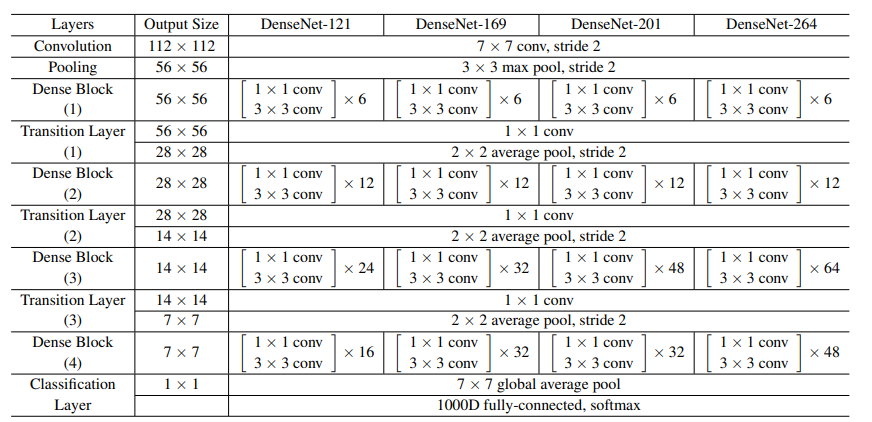
\includegraphics[width=1\linewidth]{images/densenet_archtectures_for_imagenet}
	\caption{Các kiến trúc DenseNet.}
	\label{fig:densenet_archtectures_for_imagenet}
\end{figure}

\subsection{Cài đặt mô hình DenseNet}
\begin{lstlisting}[language=Python]
def DenseNet(input_shape=(512, 512, 1),nb_dense_block=4, growth_rate=32, nb_filter=64, reduction=0.0, dropout_rate=0.0, weight_decay=1e-4, classes=1000, weights_path=None):

	eps = 1.1e-5
	
	compression = 1.0 - reduction
	
	global concat_axis
	concat_axis = 3
	img_input = Input(shape=input_shape, name='data')
	
	# From architecture for ImageNet (Table 1 in the paper)
	nb_filter = 64
	nb_layers = [6,12,24,16] # For DenseNet-121
	
	# Initial convolution
	x = ZeroPadding2D((3, 3), name='conv1_zeropadding')(img_input)
	x = Convolution2D(nb_filter, 7, 7, subsample=(2, 2), name='conv1', bias=False)(x)
	x = batch_normalization(epsilon=eps, axis=concat_axis, name='conv1_bn')(x)
	x = Activation('relu', name='relu1')(x)
	x = ZeroPadding2D((1, 1), name='pool1_zeropadding')(x)
	x = MaxPooling2D((3, 3), strides=(2, 2), name='pool1')(x)
	
	# Add dense blocks
	for block_idx in range(nb_dense_block - 1):
	stage = block_idx+2
	x, nb_filter = dense_block(x, stage, nb_layers[block_idx], nb_filter, growth_rate, dropout_rate=dropout_rate, weight_decay=weight_decay)
	
	# Add transition_block
	x = transition_block(x, stage, nb_filter, compression=compression, dropout_rate=dropout_rate, weight_decay=weight_decay)
	nb_filter = int(nb_filter * compression)
	
	final_stage = stage + 1
	x, nb_filter = dense_block(x, final_stage, nb_layers[-1], nb_filter, growth_rate, dropout_rate=dropout_rate, weight_decay=weight_decay)
	
	x = batch_normalization(epsilon=eps, axis=concat_axis, name='conv'+str(final_stage)+'_blk_bn')(x)
	x = Activation('relu', name='relu'+str(final_stage)+'_blk')(x)
	x = GlobalAveragePooling2D(name='pool'+str(final_stage))(x)
	
	x = Dense(classes, name='fc6')(x)
	x = Activation('softmax', name='prob')(x)
	
	model = Model(img_input, x, name='densenet')
	
	if weights_path is not None:
	model.load_weights(weights_path)
	
	return model
	
	
def conv_block(x, stage, branch, nb_filter, dropout_rate=None, weight_decay=1e-4):
	eps = 1.1e-5
	conv_name_base = 'conv' + str(stage) + '_' + str(branch)
	relu_name_base = 'relu' + str(stage) + '_' + str(branch)
	
	# 1x1 Convolution (Bottleneck layer)
	inter_channel = nb_filter * 4  
	x = batch_normalization(epsilon=eps, axis=concat_axis, name=conv_name_base+'_x1_bn')(x)
	x = Activation('relu', name=relu_name_base+'_x1')(x)
	x = Convolution2D(inter_channel, 1, 1, name=conv_name_base+'_x1', bias=False)(x)
	
	if dropout_rate:
	x = Dropout(dropout_rate)(x)
	
	# 3x3 Convolution
	x = batch_normalization(epsilon=eps, axis=concat_axis, name=conv_name_base+'_x2_bn')(x)
	x = Activation('relu', name=relu_name_base+'_x2')(x)
	x = ZeroPadding2D((1, 1), name=conv_name_base+'_x2_zeropadding')(x)
	x = Convolution2D(nb_filter, 3, 3, name=conv_name_base+'_x2', bias=False)(x)
	
	if dropout_rate:
	x = Dropout(dropout_rate)(x)
	
	return x
	
	
def transition_block(x, stage, nb_filter, compression=1.0, dropout_rate=None, weight_decay=1E-4):
	eps = 1.1e-5
	conv_name_base = 'conv' + str(stage) + '_blk'
	relu_name_base = 'relu' + str(stage) + '_blk'
	pool_name_base = 'pool' + str(stage) 
	
	x = batch_normalization(epsilon=eps, axis=concat_axis, name=conv_name_base+'_bn')(x)
	x = Activation('relu', name=relu_name_base)(x)
	x = Convolution2D(int(nb_filter * compression), 1, 1, name=conv_name_base, bias=False)(x)
	
	if dropout_rate:
	x = Dropout(dropout_rate)(x)
	
	x = AveragePooling2D((2, 2), strides=(2, 2), name=pool_name_base)(x)
	
	return x
	
	
def dense_block(x, stage, nb_layers, nb_filter, growth_rate, dropout_rate=None, weight_decay=1e-4, grow_nb_filters=True):
	concat_feat = x
	
	for i in range(nb_layers):
	branch = i+1
	x = conv_block(concat_feat, stage, branch, growth_rate, dropout_rate, weight_decay)
	concat_feat = merging([concat_feat, x], mode='concat', concat_axis=concat_axis, name='concat_'+str(stage)+'_'+str(branch))
	
	if grow_nb_filters:
	nb_filter += growth_rate
	
	return concat_feat, nb_filter
\end{lstlisting}

\subsection{Ưu nhược điểm của mô hình DenseNet}
\textbf{Ưu điểm:}
\begin{itemize}
	\item Giải quyết khá tốt vấn đề vanishing-gradient của các mạng CNN thuần.
	\item Cải thiện sự truyền tải đặc trưng giữa các lớp cả về phía trước cũng như phía sau.
	\item Giảm đáng kể số lượng tham số.
	\item Khuyến khích sử dụng lại các đặc trưng.
\end{itemize}
\textbf{Nhược điểm:}
\begin{itemize}
	\item Kết nối quá mức không chỉ làm giảm hiệu suất tính toán và hiệu quả tham số của mạng mà còn làm cho các mạng dễ bị overfitting. \cite{densenet_disadvantage}
\end{itemize}
	 
	 
